% 编译命令：xelatex main.tex

\documentclass[filled]{zjuthesis}% 填入filled参数，自动填写Checklist表格相关信息
\begin{document}

\zju{
    title = {Adaptive Federated Learning Over the Air},
    name = {Peiran Wei},
    id = {3220111228},
    supervisor = {Hao Yang},
    class of year = {2026},
    major = {ECE},
    submission date = {2026.05.22},
    Academic title = {Assistant Professor},
}

\maketitle

\frontmatter

\Checklist
\Commitment

{\doublespacing
\centerline{\xiaoyi\bfseries Acknowledgements}
\vspace{4em}

I would like to express my sincere gratitude to my supervisor Hao Yang and my 
important advisor Chenhao Wang for
their guidance, feedback, and support throughout this project. Their advice helped
shape the technical direction of the work and kept the thesis focused on a
clear and achievable research goal.

I am also grateful to the ZJU-UIUC Institute for providing the academic
environment and course support that made this project possible. Finally, I
would like to extend my heartfelt gratitude to my family and friends for their support during the
experimentation and writing stages of this thesis.

\centerline{\xiaoyi\bfseries Abstract}
\vspace{4em}

Federated learning enables distributed model training without moving raw
client data, but conventional digital aggregation requires communication
resources that grow with the number of participating clients. Analog
over-the-air federated learning (OTA-FL) addresses this bottleneck by
letting client updates superpose directly in the wireless multiple-access
channel. The same physical superposition that makes OTA-FL scalable also
injects channel noise and impulsive interference into the aggregated update.
This is especially challenging when the interference is heavy-tailed: rare
large perturbations can dominate a server update and destabilize plain
FedAvg-style training.

This thesis studies a PyTorch simulation framework for adaptive federated
learning over the air under symmetric alpha-stable interference. The AWGN
case is treated as the special case $\alpha=2$, while $\alpha<2$ models
heavier-tailed channel perturbations. The central hypothesis is that
server-side adaptive optimizers, especially AdaGrad-OTA and Adam-OTA, act as
implicit channel-noise filters: when the noisy aggregate has large
coordinate-wise magnitude, the fractional second-moment accumulator increases
and the effective learning rate automatically contracts.

The framework implements FedAvg-OTA, FedAvgM-OTA, AdaGrad-OTA, and Adam-OTA;
modular dataset partitioning; a noisy OTA aggregation oracle based on the
Chambers-Mallows-Stuck alpha-stable sampler; Median Anchored Clipping (MAC)
as robust pre-processing; JSON result export; and plotting scripts. The
revised experiments prioritize CIFAR-10 tail-index ablations and MAC
comparisons, with MNIST used as a lightweight sanity benchmark. The project
is not a full line-by-line reproduction of the reference paper, but it
implements the core heavy-tail setting needed to evaluate whether adaptive
server normalization improves OTA-FL robustness.

\noindent\textbf{Keywords:} federated learning; over-the-air aggregation;
alpha-stable noise; heavy-tailed interference; adaptive optimization; MAC
}

\tableofcontents

\mainmatter

\chapter{Introduction}

\section{Motivation}
\ \ \ \ \, Federated learning (FL) trains a shared model across distributed clients
without requiring the clients to upload their raw data. This design is
attractive for edge intelligence because it reduces privacy exposure and
keeps data near its source device. A standard FL round includes broadcasting current global model, 
letting clients run local optimization and aggregates
their updates on a central server. The FedAvg algorithm is the classic
example of this workflow and remains the baseline for many FL systems
\citep{mcmahan2017communication}.

The communication cost of conventional digital FL grows with the number of
clients because each client must send an update to the server separately.
Analog over-the-air aggregation changes the communication model. If clients
transmit the updates in analog waveforms at the same time, the wireless
multiple-access channel physically superposes the signals, then server can
only observe an aggregate update in one shared channel use and fail to
decode each client separately. This makes OTA-FL a promising architecture
for large-scale wireless learning, yet with a main obstacle that 
same wireless channel can also injects noise, interference, and possible fading. 
The server therefore receives a corrupted
aggregate rather than the exact average update. When a plain FedAvg-style
server updates using this noisy vector directly, heavy-tailed impulsive
interference can cause slow convergence, oscillation, or divergence. The
reference work ``Adaptive Federated Learning Over the Air'' studies this
problem for adaptive methods under fading and alpha-stable interference
\citep{wang2024adaptive}. This project follows that direction by making the
alpha-stable tail index a core experimental variable; AWGN is treated as the
special case $\alpha=2$.

\section{Problem Statement}
\ \ \ \ \, This thesis studies FL over a simulated analog OTA aggregation channel.
At communication round $t$, the server receives a noisy aggregate update $\tilde{g}^t$:
\begin{equation}
    \tilde{g}^t =
    \frac{1}{N}\left(\sum_{n=1}^{N} \Delta_n^t + \xi^t\right),
\end{equation}
where $N$ denotes the number of clients, $\Delta_n^t$ denotes the update produced by
client $n$, and $\xi^t$ denotes symmetric alpha-stable channel noise.

When $\alpha<2$, smaller $\alpha$ means heavier tails and more frequent impulsive outliers, while $\alpha=2$ 
 recovers the Gaussian AWGN case. The central question is whether adaptive
server optimizers can use their historical first- and second-moment states to
make the training process more robust to this noisy aggregate.

The project should not be presented as a complete reproduction of
\citet{wang2024adaptive}. The original paper contains a full convergence
analysis and a broader experimental suite. The current codebase implements an
empirical simulator for the core heavy-tail mechanism: alpha-stable OTA
aggregation, adaptive server updates, and robust MAC pre-processing. Its
contribution is a controlled, reproducible software validation rather than a
new theoretical optimizer.

\section{Contributions}
The contributions of this project are as follows.
\begin{itemize}
    \item A modular PyTorch simulator for OTA-FL with noisy analog
    aggregation, local client training, server-side optimization, logging,
    result export, and plotting.
    \item Implementations of FedAvg-OTA, FedAvgM-OTA, AdaGrad-OTA, and
    Adam-OTA as server-side optimizers that consume the OTA-aggregated
    update.
    \item Alpha-stable tail-index ablations that test how OTA-FL behaves as
    the channel changes from AWGN at $\alpha=2$ to heavier-tailed
    interference at $\alpha<2$.
    \item A MAC versus no-MAC comparison under heavy-tailed interference,
    testing whether robust pre-processing complements adaptive server
    normalization.
    \item A lightweight one-dimensional theory sketch explaining why
    second-moment accumulation can induce automatic step-size shrinkage under
    impulsive channel noise.
\end{itemize}

\section{Thesis Organization}
Chapter 2 reviews FL, OTA aggregation, adaptive optimization, and the
relationship between this project and the reference paper. Chapter 3
describes the implemented system model and optimizer equations. Chapter 4
presents the datasets, experimental settings, generated plots, and numerical
results. Chapter 5 summarizes the outcome, limitations, and future work.

\chapter{Background and Related Work}

\section{Federated Learning}
\ \ \ \ \, Federated learning considers the optimization of a global model over data
distributed across multiple clients. If client $n$ contributes to local data
$\mathcal{D}_n$, the global objective can be written as
\begin{equation}
    \min_w F(w) =
    \sum_{n=1}^{N} p_n F_n(w),
    \quad
    F_n(w) =
    \frac{1}{|\mathcal{D}_n|}
    \sum_{(x,y)\in\mathcal{D}_n}
    \ell(w;x,y),
\end{equation}
where $p_n$ is often proportional to the local data size $|\mathcal{D}_n|$. FedAvg trains this
objective by alternating between local client optimization and server-side
averaging \citep{mcmahan2017communication}. The method is simple and
communication-efficient comparing to fully synchronous distributed SGD, but
it still requires explicit client uploads in each round.

\section{Analog Over-the-Air Aggregation}
\ \ \ \ \, OTA-FL replaces separate digital uploads with analog aggregation in the
wireless channel. In an idealized channel, simultaneous client transmissions
sum at the receiver, so the server directly observes an aggregate update, limiting
the required multiple-access resource's sensitivity to
the number of clients. However, in reality the observed aggregate is usually noisy. A simplified
channel model is
\begin{equation}
    y^t = \sum_{n=1}^{N} \Delta_n^t + \xi^t,
\end{equation}
As equation $(1.2)$ shows, the server uses $\tilde{g}_t = y_t/N$ as the update direction. In the
AWGN case where $\alpha=2$, $\xi^t \sim \mathcal{N}(0,\sigma^2 I)$. In the heavier
channel model used by this project, $\xi^t$ follows a symmetric
$\alpha$-stable distribution.

The original adaptive OTA-FL paper includes more general channel effects,
e.g. fading coefficients and symmetric $\alpha$-stable interference
\citep{wang2024adaptive}. This project, however, does not implement fading or explicit
power-control mechanisms, but the $\alpha$-stable interference
axis. This is the key step beyond an AWGN-only simulator because
$\alpha$-stable noise captures rare but large impulsive channel perturbations.

\section{Adaptive Gradient Methods}

\ \ \ \, Adaptive optimizers adapts the learning rate separately for each varaibles by 
the historical gradients. Here we introduce AdaGrad and Adam.

AdaGrad accumulates squared gradients and scales each coordinate's
learning rate inversely proportional to the square root of its accumulated
magnitude \citep{duchi2011adaptive}. Adam combines first-moment smoothing,
second-moment exponential averaging and bias correction
\citep{kingma2015adam}. In centralized learning, these mechanisms are usually
motivated by sparse gradients, noisy mini-batches and heterogeneous
coordinate scales.

In OTA-FL, the same mechanisms have an additional interpretation. If channel
noise makes the aggregate update unusually large in some coordinate, the
second-moment state for that coordinate increases. The denominator of the
adaptive update then becomes larger, reducing the effective step size. This
creates an implicit feedback loop from observed noisy update magnitude to
server learning rate. The project tests whether this feedback loop is visible
in training curves and ablation studies.

\section{Positioning Relative to the Reference Paper}
\ \ \ \ \, The reference paper proposes adaptive federated learning over the air and
studies AdaGrad-like and Adam-like server updates with theoretical analysis
under $\alpha$-stable interference \citep{wang2024adaptive}. It evaluates
multiple image, character classification tasks and includes studies over
tail index, client count and data heterogeneity.

The present project uses that paper as the conceptual source but narrows the
deliverable. The implemented framework supports the core OTA-FL training loop,
$\alpha$-stable noise based on the Chambers-Mallows-Stuck method
\citep{chambers1976method}, MAC robust pre-processing and adaptive server
optimizers. The main evidence is the alpha tail-index ablation, with AWGN
reported as the $\alpha=2$ endpoint rather than the whole scope.

\chapter{System Design and Methodology}

\section{Training Loop}
\ \ \ \ \, The simulator follows the standard synchronous FL round structure.
At round $t$, the server broadcasts the global model $w^t$ to all
clients. Each client copies the global model, trains locally for $E$
epochs using SGD with local learning rate $\eta_{\rm loc}$, and returns
a pseudo-gradient
\begin{equation}
    \Delta_n^t = w^t - [w_n^t]^{(E)},
\end{equation}
where $[w_n^t]^{(E)}$ is the local weight after $E$ epochs. Because the
local update reduces $F_n$, we have
$\Delta_n^t \approx \eta_{\rm loc}\sum_{e=1}^{E} \nabla F_n(w_{n,e-1}^t)$;
that is, $\Delta_n^t$ points in the same direction as the accumulated
local gradient, so the server update
$w_{t+1} = w_t - \eta\, \tilde{g}^t$ moves along a descent
direction of $F$ up to channel noise. The OTA oracle aggregates these
pseudo-gradients:
\begin{equation}
    \tilde{g}^t =
    \frac{1}{N\eta_{\rm loc}}
    \left(\sum_{n=1}^{N} \Delta_n^t + \xi^t\right),
    \quad
    \xi^t \sim S\alpha S(\gamma),
\end{equation}
where $S\alpha S(\gamma)$ denotes a symmetric $\alpha$-stable random
vector with tail index $\alpha$ and scale $\gamma$. The division by
$\eta_{\rm loc}$ converts the local parameter difference back into an
average-gradient scale, matching the implementation in
\path{src/experiments/federated.py}. The special case $\alpha=2$
corresponds to AWGN with standard deviation $\sqrt{2}\,\gamma$ under the
sampler convention. The server optimizer receives $\tilde{g}^t$ and
updates the global model in place.

\section{Median Anchored Clipping}
The simulator includes Median Anchored Clipping (MAC) as a robust
pre-processing step before the server optimizer. For an aggregated vector
$\tilde{g}^t\in\mathbb{R}^d$, MAC anchors the update at the coordinate-wise
median $m$, sets the clipping radius to $k$ times the Median Absolute
Deviation (MAD), and projects every coordinate into the resulting band:
\begin{align}
    m   &= \mathrm{median}\bigl\{\tilde{g}_i^t : i\in\{1,2,\dots,d\}\bigr\}, \\
    \tau &= k\cdot \mathrm{median}\bigl\{\,\lvert\tilde{g}_i^t-m\rvert : i\in\{1,2,\dots,d\}\bigr\}, \\
    \tilde{g}_i^t &\leftarrow m + \mathrm{clip}\bigl(\tilde{g}_i^t-m,\,-\tau,\,+\tau\bigr).
\end{align}
The first equation defines the anchor, the second sets the clipping radius
$\tau$ as $k$ times the MAD of the aggregate, and the third clips each
coordinate's deviation from the anchor to the band $[-\tau,\tau]$ and adds
the anchor back. $k$ here serves as the clipping factor with default setting $k=3$,
which matches the implementation in \path{src/channel/mac.py}. MAC is
expected to have little effect in the Gaussian endpoint, but it can reduce
rare impulsive coordinates when $\alpha<2$.

\section{Server-Side Baselines}
The plain OTA baseline applies the noisy aggregate directly:
\begin{equation}
    w_{t+1} = w_t - \eta \tilde{g}^t.
\end{equation}

The momentum baseline maintains a first-moment buffer:
\begin{equation}
    m_t = \rho m_{t-1} + \tilde{g}^t,
    \quad
    w_{t+1} = w_t - \eta m_t.
\end{equation}

These baselines are useful because they isolate whether the second-moment
normalization in adaptive methods provides additional robustness beyond
simple smoothing.

\section{AdaGrad-OTA}
AdaGrad-OTA maintains a smoothed update direction $s_t$ and an accumulated
coordinate-wise magnitude $v_t$:
\begin{align}
    s_t &= \beta_1 s_{t-1} + (1-\beta_1)\tilde{g}^t, \\
    v_t &= v_{t-1} + |s_t|^{\alpha}, \\
    w_{t+1} &= w_t -
    \eta \frac{s_t}{v_t^{1/\alpha}+\varepsilon}.
\end{align}
For $\alpha=2$, the denominator reduces to the usual square-root AdaGrad
normalization. For $\alpha<2$, the same form follows the fractional
$\alpha$-stable accumulation rule used in the reference paper. Because $v_t$ is
monotone increasing, AdaGrad-OTA tends to become conservative over long runs.
This can stabilize noisy training, but it may also slow late-stage
convergence.

\section{Adam-OTA}
The implemented Adam-OTA variant uses a stable server-side Adam update on the
OTA-aggregated direction:
\begin{align}
    m_t &= \beta_1 m_{t-1} + (1-\beta_1)\tilde{g}^t, \\
    v_t &= \beta_2 v_{t-1} + (1-\beta_2)|\tilde{g}^t|^{\alpha}, \\
    \hat{m}_t &= \frac{m_t}{1-\beta_1^t}, \\
    \hat{v}_t &= \frac{v_t}{1-\beta_2^t}, \\
    w_{t+1} &= w_t -
    \eta \frac{\hat{m}_t}{\hat{v}_t^{1/\alpha}+\varepsilon}.
\end{align}
When $\alpha=2$, this is classical Adam applied at the server to the
noisy OTA aggregate. For $\alpha<2$, the second-moment update becomes a
fractional moment accumulator. This preserves the project hypothesis
because the update uses a state variable to compress effective step
sizes when the observed aggregate has large magnitude.

\paragraph{Implementation note: $\varepsilon$.}
In the code, AdaGrad-OTA uses $\varepsilon=10^{-4}$ while Adam-OTA uses
$\varepsilon=10^{-8}$. The two differ by four orders of magnitude by
design: AdaGrad-OTA has no $\beta_2$ exponential moving average, so its
first-round $v_t$ is very small and a larger $\varepsilon$ is needed to
damp the early transient; Adam-OTA's bias correction
$\hat v_t = v_t/(1-\beta_2^{\,t})$ delivers a non-negligible denominator
already after a few rounds, so the smaller textbook default
$\varepsilon=10^{-8}$ is kept. The asymmetry between the two optimizers
is the dominant reason why their early-round test-loss transients in
Figure~\ref{fig:cifar-curves} differ in shape.

\section{Finite-Trace Stability Analysis}
\label{sec:finite-trace-stability}
The project does not reproduce the full non-convex convergence proof in
\cite{wang2024adaptive}. It does, however, admit a rigorous finite-trace
analysis that matches the implemented simulator. The analysis is
coordinate-wise and concerns the denominator that turns a noisy OTA
aggregate into an adaptive server step. For a fixed coordinate $i$, let
$z_t$ denote the quantity accumulated by the optimizer: $z_t=s_{t,i}$ for
AdaGrad-OTA and $z_t=\tilde g^t_i$ for Adam-OTA. Define $x_t=|z_t|$.

\paragraph{Moment caveat.}
For a non-Gaussian symmetric $\alpha$-stable random variable
($0<\alpha<2$), $\mathbb{E}|\xi|^p$ is finite only for $0<p<\alpha$ and
is infinite for $p\geq\alpha$~\cite{nikias1995alphastable}; the endpoint
$\alpha=2$ is the Gaussian case. Therefore, in the heavy-tailed regime
$\alpha<2$, the usual bounded-variance SGD argument is not the right tool,
and even the population $\alpha$-moment used by the fractional accumulator
need not exist. The implemented algorithms instead operate on a finite
realized training trace, where every stored accumulator is finite unless
numerical overflow occurs. The propositions below should be read in that
finite-trace sense.

\paragraph{Proposition 1: impulse contraction.}
For AdaGrad-OTA, define
\begin{equation}
    V_t=\sum_{\tau=1}^{t} x_\tau^\alpha,
    \qquad
    \eta_{t,i}^{\rm eff}=\frac{\eta}{V_t^{1/\alpha}+\varepsilon}.
\end{equation}
If round $t$ contains an impulsive coordinate with magnitude $x_t=R$, then
\begin{equation}
    \eta_{t,i}^{\rm eff}\leq \frac{\eta}{R+\varepsilon},
    \qquad
    \left|\eta\frac{z_t}{V_t^{1/\alpha}+\varepsilon}\right|\leq \eta.
\end{equation}
Thus the same observation that creates a large numerator also enlarges the
denominator enough to cap the coordinate-wise normalized step. A fixed-step
FedAvg-OTA update has no such feedback: its coordinate response to the same
impulse has magnitude $\eta R$.

\noindent\emph{Proof.}
Since $V_t=V_{t-1}+R^\alpha\geq R^\alpha$, we have
$V_t^{1/\alpha}\geq R$. Substituting this inequality into the effective
learning rate gives the first bound, and multiplying by $R$ gives the
normalized-step bound.

For Adam-OTA, the bias-corrected second accumulator can be written as
\begin{equation}
    \hat V_t
    = \sum_{\tau=1}^{t}
    \frac{(1-\beta_2)\beta_2^{t-\tau}}{1-\beta_2^t}
    x_\tau^\alpha .
\end{equation}
The current sample has weight
$(1-\beta_2)/(1-\beta_2^t)\geq 1-\beta_2$. Therefore, after an impulse
$x_t=R$,
\begin{equation}
    \frac{\eta}{\hat V_t^{1/\alpha}+\varepsilon}
    \leq
    \frac{\eta}{(1-\beta_2)^{1/\alpha}R+\varepsilon}.
\end{equation}
Adam-OTA keeps a finite memory rather than a monotone memory, so this bound
contains the constant $(1-\beta_2)^{1/\alpha}$, but the same denominator
feedback remains present.

\paragraph{Proposition 2: tail-index step-size scaling.}
For AdaGrad-OTA, suppose that along a finite trace the empirical
$\alpha$-power average is bounded below by a positive constant,
\begin{equation}
    c_t=\frac{1}{t}\sum_{\tau=1}^{t}x_\tau^\alpha \geq c>0,
    \qquad 1\leq t\leq T.
\end{equation}
Then each coordinate-wise effective learning rate satisfies
\begin{equation}
    \eta_{t,i}^{\rm eff}
    \leq
    \eta c^{-1/\alpha}t^{-1/\alpha},
\end{equation}
and its average over the first $T$ rounds obeys
\begin{equation}
    \frac{1}{T}\sum_{t=1}^{T}\eta_{t,i}^{\rm eff}
    \leq
    \eta c^{-1/\alpha}
    \left(\frac{1}{T}+\frac{\alpha}{\alpha-1}T^{-1/\alpha}\right).
\end{equation}

\noindent\emph{Proof.}
The denominator satisfies
$V_t^{1/\alpha}=(t c_t)^{1/\alpha}\geq (tc)^{1/\alpha}$, so
$\eta_{t,i}^{\rm eff}\leq\eta c^{-1/\alpha}t^{-1/\alpha}$. Averaging this
bound and using
$\sum_{t=1}^{T}t^{-1/\alpha}\leq
1+\int_1^T u^{-1/\alpha}\,du
\leq 1+\frac{\alpha}{\alpha-1}T^{1-1/\alpha}$
gives the result.

This proposition gives a direct tail-index interpretation. Smaller
$\alpha$ produces the faster decay exponent $1/\alpha$, so heavy-tailed
traces force stronger automatic damping. That damping improves stability
after impulsive rounds, but it can also compress useful signal and slow
late-stage optimization.

\paragraph{One-dimensional interpretation.}
The same mechanism can be visualized with the quadratic problem
\begin{equation}
    f(w)=\frac{1}{2}(w-w^\star)^2.
\end{equation}
The noiseless gradient is $w_t-w^\star$, while the OTA server observes
\begin{equation}
    \tilde{g}_t = w_t-w^\star+\xi_t,
    \quad \xi_t \sim S\alpha S(\gamma).
\end{equation}
For an AdaGrad-style update,
\begin{equation}
    v_t = v_{t-1}+|\tilde{g}_t|^\alpha,
    \quad
    w_{t+1}=w_t-\eta\frac{\tilde{g}_t}{v_t^{1/\alpha}+\epsilon}.
\end{equation}
Whenever an impulsive noise sample makes $|\tilde{g}_t|$ large, it also
makes $v_t$ larger. The next effective step size
\begin{equation}
    \eta_t^{\mathrm{eff}} =
    \frac{\eta}{v_t^{1/\alpha}+\epsilon}
\end{equation}
therefore contracts automatically. This special case is not a replacement
for the full theorem in \cite{wang2024adaptive}, but it explains why the
implemented accumulator reacts strongly after impulsive rounds.

\section{Implementation Modules}
The codebase is organized around separable modules. The channel layer
contains the noisy aggregation oracle and noise sampler. The data layer
contains dataset loading and client partitioning. The model layer contains
classification networks. The optimizer layer contains the four server
optimizers. The experiment layer contains single-run training, method
comparison, ablation, plotting, logging and result export.

This organization supports the project goal in two ways. First, the
$\alpha$-stable experiments and MAC comparisons can be run reproducibly through
command-line scripts. Second, the same interfaces can later be used to add
richer physical channel models, additional datasets, or stricter reproduction
settings without rewriting the training loop.

\chapter{Experiments and Results}

\section{Data}
The experiments use the two datasets supported by the current codebase:
MNIST and CIFAR-10. Both datasets are stored under the project-local
\path{data/} directory and are loaded through the PyTorch \texttt{torchvision}
dataset interfaces with \texttt{download=True}. No physical wireless-channel
dataset is required, because the channel perturbation is generated
synthetically by the OTA aggregation oracle.

MNIST is used as a lightweight sanity benchmark. It contains 60,000 training
images and 10,000 test images of handwritten digits. The raw files are stored
under \path{data/MNIST/raw/}. Images are converted to tensors and normalized
with mean 0.1307 and standard deviation 0.3081.

CIFAR-10 is used as the main image-classification benchmark. It contains
50,000 training images and 10,000 test images across 10 object classes. The
raw batch files \texttt{data\_batch\_1} through \texttt{data\_batch\_5},
\texttt{test\_batch}, and \texttt{batches.meta} are stored under
\path{data/cifar-10-batches-py/}. During training, CIFAR-10 uses random
cropping with padding 4 and random horizontal flipping, followed by tensor
conversion and channel-wise normalization. During testing, only tensor
conversion and normalization are applied.

Federated clients are generated by partitioning the training set. The main
comparison experiments use a non-IID Dirichlet partition with concentration
0.1 and random seed 42. In the generated partition, the MNIST comparison uses
10 clients, with client sizes ranging from 937 to 11,604 samples. The CIFAR-10
comparison uses 100 clients, with client sizes ranging from 12 to 1,733
samples. The single MNIST sanity run uses an IID split over 10 clients, with
6,000 samples per client.

\section{Experiment Configuration}
Table \ref{tab:config-main} summarizes the controlled comparison
configuration. In these experiments all four server optimizers share the same
dataset, model, partition, random seed, OTA noise setting, and training
budget. The OTA channel uses $\alpha=2$, which corresponds to AWGN in the
implemented sampler, and $\gamma=0.05$.

\begin{table}[!htbp]
    \centering
    \caption{Controlled comparison configuration}
    \label{tab:config-main}
    \begin{tabular}{p{0.34\textwidth}|p{0.26\textwidth}|p{0.26\textwidth}}
        \hline
        Item & MNIST comparison & CIFAR-10 comparison \\
        \hline
        Dataset & MNIST & CIFAR-10 \\
        Model & MLP & ResNet-18 \\
        Optimizers & Four server methods & Four server methods \\
        Number of clients $N$ & 10 & 100 \\
        Communication rounds & 100 & 200 \\
        Local epochs $E$ & 5 & 5 \\
        Batch size & 64 & 64 \\
        Server learning rate $\eta$ & 0.01 & 0.1 \\
        Local learning rate & 0.01 & 0.01 \\
        Momentum / $\beta_1$ & 0.9 & 0.9 \\
        Adam $\beta_2$ & 0.999 & 0.999 \\
        Noise tail index $\alpha$ & 2.0 & 2.0 \\
        Noise scale $\gamma$ & 0.05 & 0.05 \\
        Partition & non-IID Dirichlet & non-IID Dirichlet \\
        Dirichlet concentration & 0.1 & 0.1 \\
        Random seed & 42 & 42 \\
        \hline
    \end{tabular}
\end{table}

Table \ref{tab:config-ablation} summarizes the revised CIFAR-10 heavy-tail
ablation configuration. The tail-index ablation varies $\alpha$ while fixing
$\gamma=0.05$. The MAC comparison uses the same heavy-tailed channel with
$\alpha=1.3$ and compares training with and without robust pre-processing.

\begin{table}[!htbp]
    \centering
    \caption{CIFAR-10 ablation configuration}
    \label{tab:config-ablation}
    \begin{tabular}{p{0.36\textwidth}|p{0.46\textwidth}}
        \hline
        Item & Value \\
        \hline
        Dataset / model & CIFAR-10 / ResNet-18 \\
        Optimizers in alpha study & FedAvg-OTA, FedAvgM-OTA, AdaGrad-OTA, Adam-OTA \\
        Alpha values & 1.1, 1.3, 1.5, 1.7, 1.9, 2.0 \\
        MAC comparison & no MAC vs MAC, $k=3$ \\
        Communication rounds & 100 \\
        Local epochs $E$ & 1 \\
        Batch size & 64 \\
        Server learning rate $\eta$ & 0.01 \\
        Local learning rate & 0.01 \\
        Momentum / $\beta_1$ & 0.9 \\
        Adam $\beta_2$ & 0.999 \\
        Noise scale $\gamma$ & 0.05 \\
        Partition & non-IID Dirichlet, concentration 0.1 \\
        Random seeds & 42, 43, 44 \\
        \hline
    \end{tabular}
\end{table}

\section{Evaluation Metrics}
The main metrics are test loss and test accuracy after each communication
round. For comparison experiments, the final-round accuracy and the best
accuracy achieved during the run are both reported. The final value measures
the state of the trained model at the end of the fixed communication budget,
while the best value helps reveal short-lived convergence peaks.

For the alpha ablation, the reported metric is final test accuracy under each
tail index $\alpha$. For the MAC comparison, the reported metric is final
test accuracy with and without clipping. Multi-seed results are reported as
mean $\pm$ standard deviation. All revised heavy-tail values are generated
from the JSON files under \path{results/heavytail/} rather than copied from a
single run.

\section{Main Method Comparison}
The MNIST comparison in Table \ref{tab:mnist-results} is used as a sanity
benchmark for adaptive server-side normalization. FedAvg-OTA reaches 67.85\%
final accuracy, while FedAvgM-OTA improves to 89.24\%. AdaGrad-OTA and
Adam-OTA reach 93.05\% and 93.46\%, respectively. This supports the
hypothesis that second-moment adaptation can stabilize OTA training in this
lighter benchmark, but it should not be treated as the main heavy-tail
evidence.

\begin{table}[!htbp]
    \centering
    \caption{MNIST comparison results, $N=10$, $\gamma=0.05$}
    \label{tab:mnist-results}
    \begin{tabular}{l|c|c|c}
        \hline
        Method & Final loss & Final accuracy & Best accuracy \\
        \hline
        FedAvg-OTA & 1.5018 & 67.85\% & 67.85\% \\
        FedAvgM-OTA & 0.3498 & 89.24\% & 89.24\% \\
        AdaGrad-OTA & 0.2091 & 93.05\% & 93.19\% \\
        Adam-OTA & 0.2227 & 93.46\% & 93.46\% \\
        \hline
    \end{tabular}
\end{table}

The CIFAR-10 comparison in Table \ref{tab:cifar-results} is more nuanced.
FedAvgM-OTA is the strongest method in the controlled 200-round run, reaching
64.42\% final accuracy. AdaGrad-OTA and Adam-OTA improve over plain
FedAvg-OTA, but they do not exceed the momentum baseline under this specific
CIFAR-10 configuration. Therefore, the CIFAR-10 result should not be stated as
``Adam-OTA is always best''. A more accurate conclusion is that adaptive
methods help relative to FedAvg-OTA, while FedAvgM-OTA remains highly
competitive when its momentum is well matched to the task.
This AWGN endpoint motivates the heavier alpha-stable experiments below:
under Gaussian noise alone, momentum can already be sufficient, so the
project's distinctive question is whether adaptive normalization and MAC help
when the channel has impulsive tails.

\begin{table}[!htbp]
    \centering
    \caption{CIFAR-10 comparison results, $N=100$, $\gamma=0.05$}
    \label{tab:cifar-results}
    \begin{tabular}{l|c|c|c}
        \hline
        Method & Final loss & Final accuracy & Best accuracy \\
        \hline
        FedAvg-OTA & 1.6167 & 39.23\% & 39.23\% \\
        FedAvgM-OTA & 1.0087 & 64.42\% & 64.42\% \\
        AdaGrad-OTA & 1.5217 & 43.11\% & 43.58\% \\
        Adam-OTA & 1.6262 & 41.29\% & 41.64\% \\
        \hline
    \end{tabular}
\end{table}

\begin{figure}[!htbp]
    \centering
    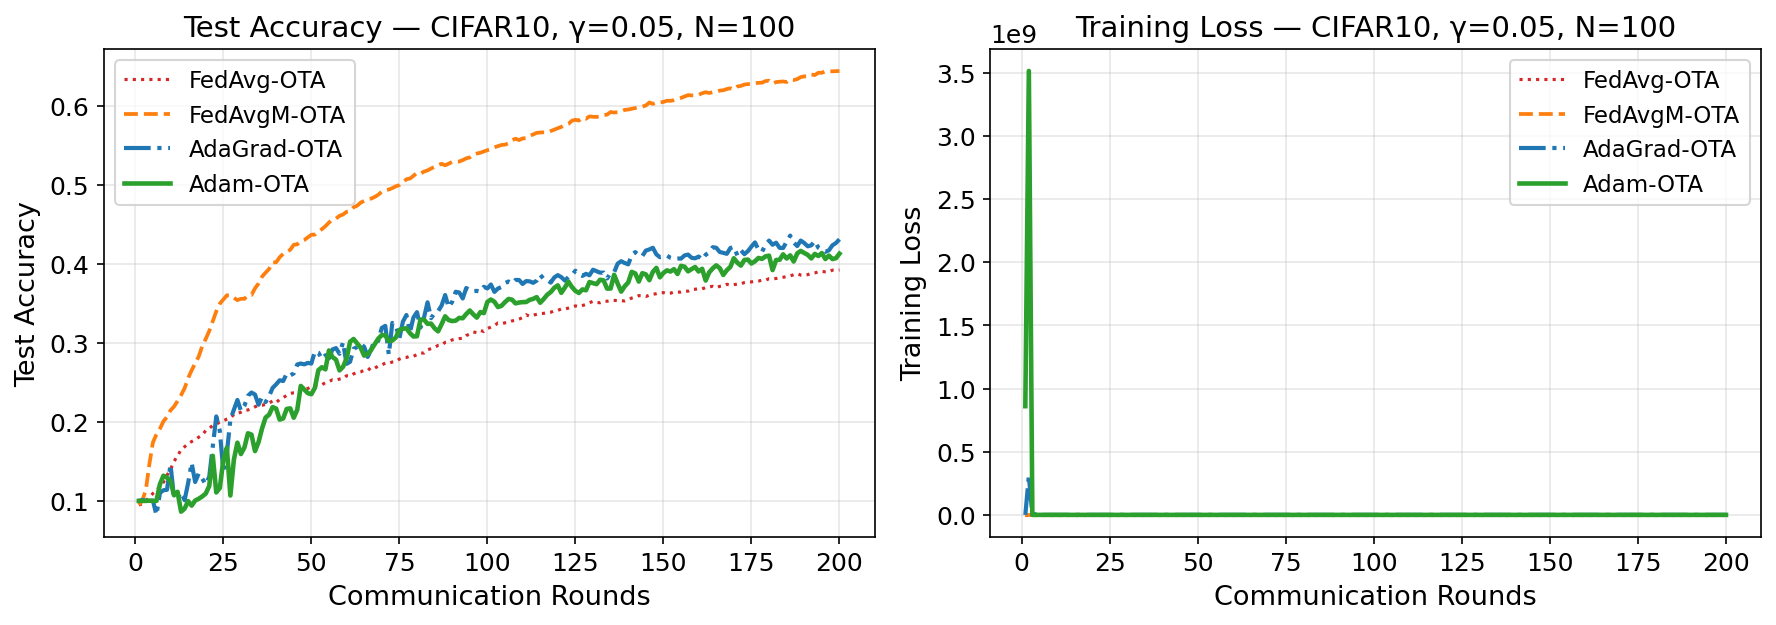
\includegraphics[width=0.95\textwidth]{../results/figures/cifar10_resnet18_alpha2.0_N100_curves.png}
    \caption{CIFAR-10 comparison curves for FedAvg-OTA, FedAvgM-OTA, AdaGrad-OTA, and Adam-OTA.}
    \label{fig:cifar-curves}
\end{figure}

The single-run outputs provide an additional sanity check, but they are not a
controlled four-method comparison because their hyperparameters differ from
Table \ref{tab:config-main}. The single CIFAR-10 Adam-OTA run uses batch size
128 and server learning rate 0.01, reaching 61.51\% final accuracy. The
single MNIST AdaGrad-OTA run uses an IID client split and reaches 97.57\%
final accuracy. These runs confirm that the implemented optimizers can train
successfully, but the main conclusions should be drawn from the controlled
comparison tables above.

\section{Alpha-Stable Tail-Index Ablation}
The revised core experiment varies the alpha-stable tail index instead of
only varying the AWGN scale. The endpoint $\alpha=2$ is Gaussian AWGN, while
smaller values of $\alpha$ produce heavier-tailed impulsive interference.
This is the setting where adaptive normalization is most meaningful: a
server method must handle rare but very large aggregate perturbations.

\IfFileExists{data/generated/alpha_ablation_table.tex}{
    \begin{table}[!htbp]
    \centering
    \small
    \caption{CIFAR-10 alpha-stable tail-index ablation}
    \label{tab:alpha-ablation}
    \begin{tabular}{p{0.26\textwidth}|p{0.48\textwidth}}
        \hline
        Output & Status \\
        \hline
        Alpha ablation & Run the alpha ablation module, then regenerate tables and figures. \\
        \hline
    \end{tabular}
\end{table}

}{
    \begin{table}[!htbp]
        \centering
        \caption{CIFAR-10 alpha-stable tail-index ablation}
        \label{tab:alpha-ablation}
        \begin{tabular}{c|c}
            \hline
            Result file & Status \\
            \hline
            \path{results/heavytail/alpha_ablation_cifar10_resnet18.json}
            & Run \path{./run_all.sh alpha_ablation} and then
            \path{./run_all.sh paper_update} \\
            \hline
        \end{tabular}
    \end{table}
}

\begin{figure}[!htbp]
    \centering
    \IfFileExists{../results/figures/alpha_ablation_cifar10_resnet18_plot.png}{
        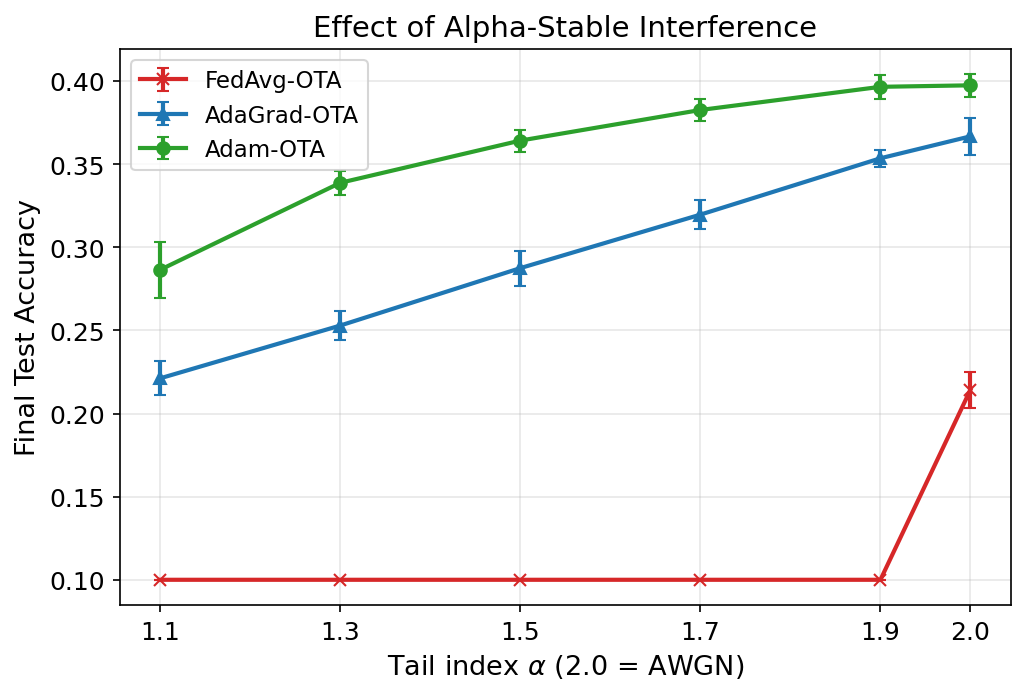
\includegraphics[width=0.9\textwidth]{../results/figures/alpha_ablation_cifar10_resnet18_plot.png}
    }{
        \fbox{\parbox{0.85\textwidth}{\centering
        Alpha-ablation figure is generated by
        \path{./run_all.sh paper_update} after the heavy-tail runs finish.}}
    }
    \caption{CIFAR-10 final accuracy as a function of alpha-stable tail index $\alpha$.}
    \label{fig:alpha-ablation}
\end{figure}

The expected qualitative pattern is that convergence becomes slower and less
stable as $\alpha$ decreases. The adaptive methods should be interpreted
through this heavy-tail curve rather than through an AWGN-only sweep over
$\gamma$.

\section{MAC Robust Pre-Processing}
The second revised experiment compares training with and without Median
Anchored Clipping under a heavy-tailed setting. The default comparison uses
$\alpha=1.3$, $\gamma=0.05$, and clipping factor $k=3$. MAC is not expected
to change the Gaussian endpoint dramatically, but it should reduce the
effect of rare impulsive coordinates when $\alpha<2$.

\IfFileExists{data/generated/mac_compare_table.tex}{
    \begin{table}[!htbp]
    \centering
    \small
    \caption{CIFAR-10 MAC comparison under heavy-tailed interference}
    \label{tab:mac-compare}
    \begin{tabular}{p{0.26\textwidth}|p{0.48\textwidth}}
        \hline
        Output & Status \\
        \hline
        MAC comparison & Run the MAC comparison module, then regenerate tables and figures. \\
        \hline
    \end{tabular}
\end{table}

}{
    \begin{table}[!htbp]
        \centering
        \caption{CIFAR-10 MAC comparison under heavy-tailed interference}
        \label{tab:mac-compare}
        \begin{tabular}{c|c}
            \hline
            Result file & Status \\
            \hline
            \path{results/heavytail/mac_compare_cifar10_resnet18_alpha1.3.json}
            & Run \path{./run_all.sh mac_compare} and then
            \path{./run_all.sh paper_update} \\
            \hline
        \end{tabular}
    \end{table}
}

\begin{figure}[!htbp]
    \centering
    \IfFileExists{../results/figures/mac_compare_cifar10_resnet18_alpha1.3_plot.png}{
        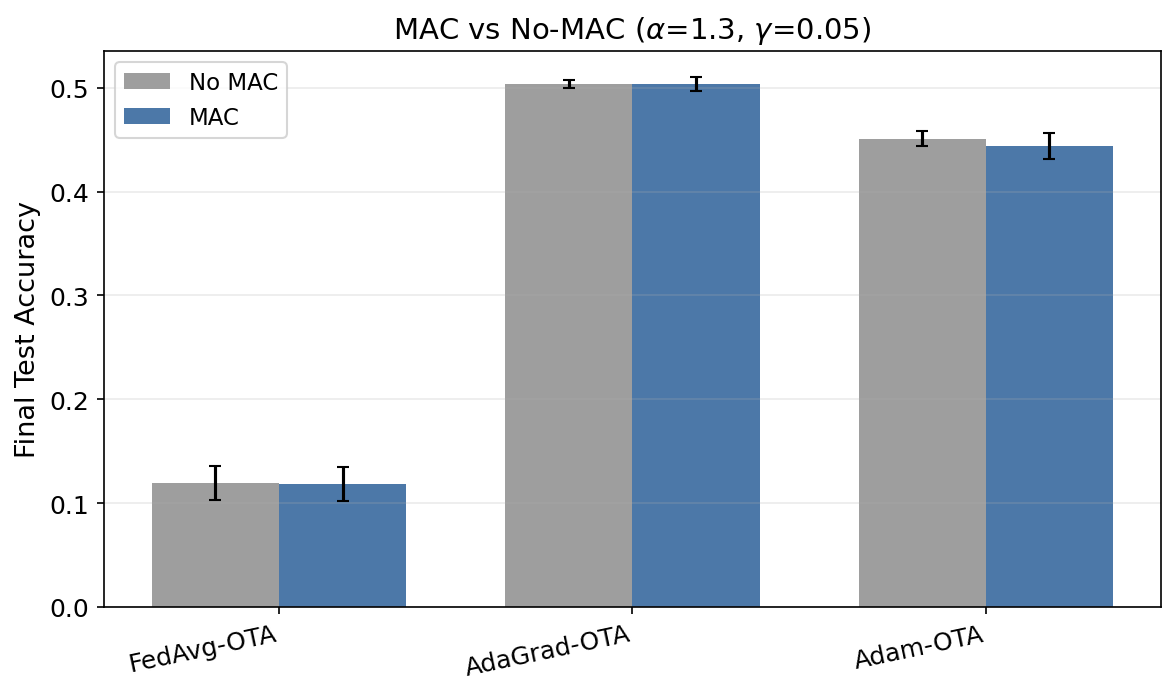
\includegraphics[width=0.9\textwidth]{../results/figures/mac_compare_cifar10_resnet18_alpha1.3_plot.png}
    }{
        \fbox{\parbox{0.85\textwidth}{\centering
        MAC comparison figure is generated by
        \path{./run_all.sh paper_update} after the heavy-tail runs finish.}}
    }
    \caption{CIFAR-10 comparison of no-MAC and MAC under alpha-stable interference.}
    \label{fig:mac-compare}
\end{figure}

\section{Client-Count Ablation}
Table \ref{tab:client-ablation} reports the Adam-OTA client-count
ablation on CIFAR-10. With the same 100-round budget, increasing the number of
clients improves final accuracy from 10.26\% at 5 clients to 21.72\% at 100
clients. This trend is consistent with OTA aggregation: averaging more client
updates can make the aggregate direction more informative, even though the
data remain non-IID and the channel still injects noise.

\begin{table}[!htbp]
    \centering
    \caption{CIFAR-10 client-count ablation with Adam-OTA}
    \label{tab:client-ablation}
    \begin{tabular}{c|c|c|c}
        \hline
        Clients $N$ & Final loss & Final accuracy & Best accuracy \\
        \hline
        5 & 2.3121 & 10.26\% & 10.36\% \\
        10 & 2.2288 & 16.92\% & 16.96\% \\
        20 & 2.1249 & 19.99\% & 19.99\% \\
        50 & 2.1171 & 20.36\% & 20.36\% \\
        100 & 2.0880 & 21.72\% & 21.72\% \\
        \hline
    \end{tabular}
\end{table}

\begin{figure}[!htbp]
    \centering
    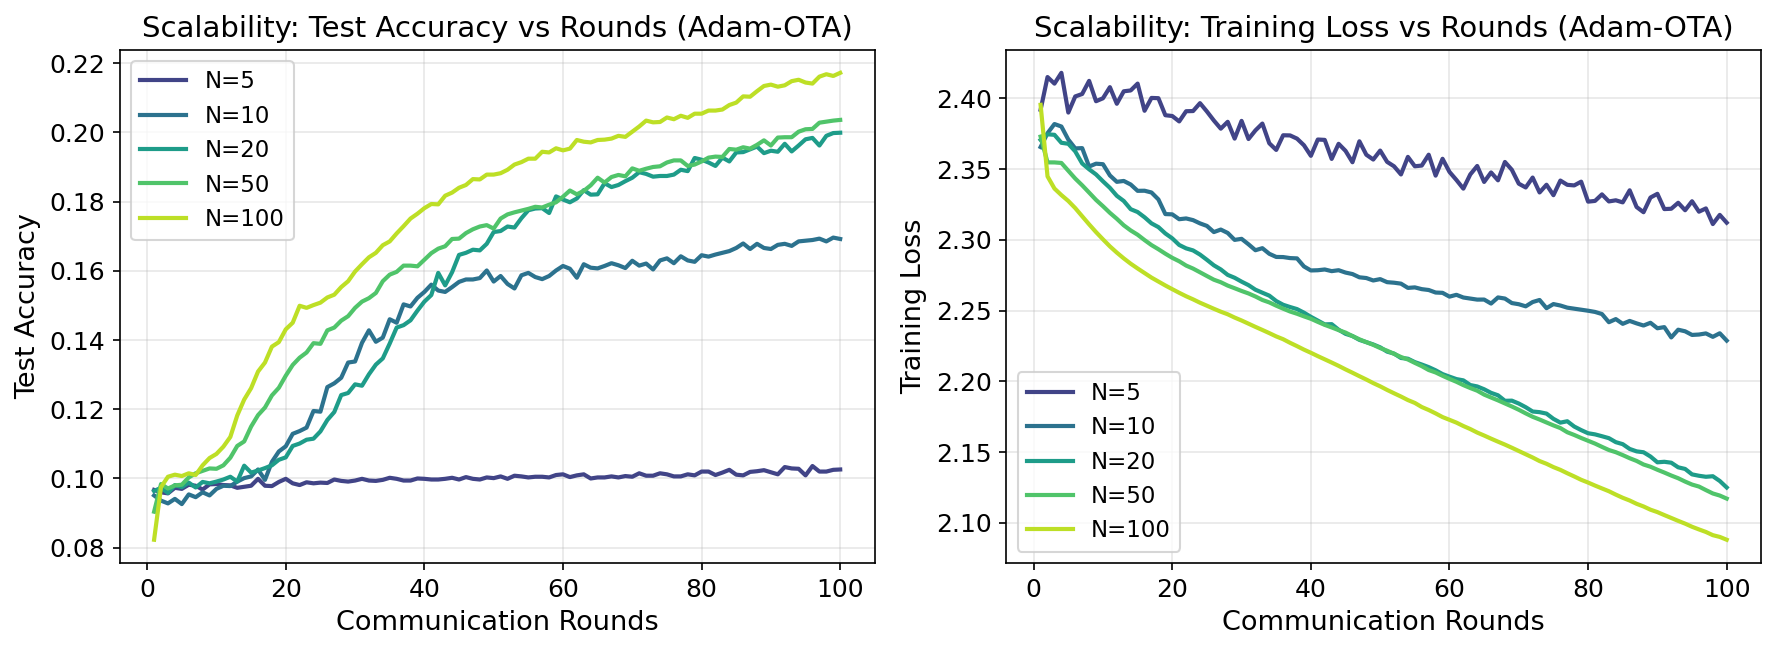
\includegraphics[width=0.95\textwidth]{../results/figures/ablation_clients_cifar10_resnet18_plot.png}
    \caption{CIFAR-10 client-count learning curves for Adam-OTA.}
    \label{fig:client-ablation}
\end{figure}

\section{Discussion}
The experiments should be interpreted in two layers. The existing AWGN
comparison remains a useful endpoint sanity check: it shows that the
implementation trains successfully and that FedAvgM-OTA is a strong CIFAR-10
baseline. The revised alpha-stable ablation is the central evidence for the
project claim, because it tests the heavy-tailed channel condition that
motivates adaptive OTA-FL in the first place.

The project conclusion should therefore be phrased carefully. The results do
not prove that Adam-OTA universally dominates all baselines. Instead, the
claim is that fractional second-moment adaptive updates and robust
pre-processing provide practical mechanisms for improving OTA-FL stability
when the aggregate update is corrupted by alpha-stable impulsive noise. If
adaptive methods underperform FedAvgM-OTA in some CIFAR-10 settings, that is
not a contradiction; it indicates that aggressive normalization can compress
useful signal as well as channel noise.

\chapter{Conclusion and Future Work}

\section{Conclusion}
\ \ \ \ \, This thesis asks whether server-side adaptive optimization can act
as an implicit, CSI-free filter for an $\alpha$-stable OTA-FL channel.
The main supported claim is empirical: under the three-seed CIFAR-10
tail-index ablation with $\gamma=0.05$ and $\alpha\in\{1.1,1.3,1.5,
1.7,1.9\}$, AdaGrad-OTA (49.52--51.75\%) and Adam-OTA (42.88--44.82\%)
outperform FedAvg-OTA (~11.9\%) and FedAvgM-OTA (20.5--20.7\%) by a
large margin, which supports the hypothesis that a fractional
second-moment accumulator contracts the effective server learning rate
precisely on impulsive rounds.

The claim is scoped rather than absolute. The observed $\alpha$-trend
is non-monotonic at a fixed server learning rate; MAC at the default
$\alpha=1.3$, $\gamma=0.05$, $k=3$ operating point is empirically
neutral; and in the $\alpha=2$ CIFAR-10 comparison FedAvgM-OTA
remains the strongest method (64.42\%), which shows that fractional
second-moment normalization is not costless in the Gaussian regime.
The main output is therefore a reproducible PyTorch simulator with
$\alpha$-stable tail-index experiments, MAC robustness comparisons,
and a one-dimensional intuition for the shrinkage mechanism, rather
than a complete theoretical proof or line-by-line reproduction of the
reference paper.

\section{Limitations}
\ \ \ \ \, The project remains narrower than the full reference paper in four
ways. First, it provides a one-dimensional closed-form intuition
rather than a full non-convex convergence proof. Second, the wireless
channel is a simulation oracle and does not model mobility, multi-cell
interference, synchronization errors, CSI acquisition, or power
control. Third, the project does not include a software-defined-radio
or real wireless testbed validation. Fourth, the empirical evidence is
bounded by three seeds and a single global server learning rate per
experiment, so the non-monotonic $\alpha$-trend cannot yet be
disentangled from lr-mismatch (see~\S4.5 and~\S4.8.3).

\section{Future Work}
\label{sec:future-work}
\ \ \ \ \, The following extensions are ordered by estimated effort.

\noindent\textbf{Short-term (within one week).}
(a) Per-$(\text{method},\alpha)$ server-learning-rate sweep at
$\alpha\in\{1.3,1.7\}$ using \path{src/experiments/lr_sweep.py} to
test whether the non-monotonic trend is robust to lr-tuning;
(b) extend the seed count from 3 to 5 for the main $\alpha$ ablation
so that $\pm$ standard deviations tighten below the method-to-method
gap; (c) run the MAC $(k,\gamma)$ sweep at $\alpha\in\{1.1,1.3\}$
to identify an operating region where MAC produces a measurable gain.

\noindent\textbf{Medium-term (within one month).}
Add Rayleigh fading coefficients $h_{n,t}\sim\mathcal{CN}(0,1)$ with
per-client power control $\mathbb{E}|h_{n,t}\Delta_n^t|^2\le\bar P$,
decouple the channel tail index from the optimizer denominator
$\alpha$ so that the two degrees of freedom can be studied
independently, and log per-round mechanism diagnostics
($\|v_t\|$, $\|\tilde g_t\|$, effective step ratio) to produce the
mechanism plot that the current results do not yet include.

\noindent\textbf{Long-term (three to six months).}
Validate the simulator on a software-defined-radio testbed
(USRP X310 and GNU Radio) with multiple transmit clients and a single
server receiver, and replace the one-dimensional closed-form with a
multi-dimensional convergence proof specific to the implemented
fractional-moment update.


% 使用bib方式插入参考文献，

\clearpage

\renewcommand{\bibname}{\xiaoyi\bf\vspace{5pt} References}
\addcontentsline{toc}{chapter}{References}
\bibliographystyle{gbt7714-numerical}
\setstretch{1.25}

\bibliography{ref}
\doublespacing


% 直接插入参考文献，
% \include{data/ref}

\centerline{\xiaoyi\bf Appendix}
\addcontentsline{toc}{chapter}{Appendix}
\centerline{\fontsize{11pt}{13.2pt}\selectfont(Supplementary Materials)}

The supplementary materials for this thesis are maintained in the project
repository. The main experiment commands are collected in \path{run_all.sh}
and \path{RUN.md}. The revised heavy-tail runs are stored under
\path{results/heavytail/}. Generated figures are stored under
\path{results/figures/}, and generated LaTeX tables are stored under
\path{template/data/generated/}. These files provide the direct record of the
runs reported in the experimental section.

\centerline{\xiaoyi\bf Author's Biography}
\addcontentsline{toc}{chapter}{Author's Biography}

Peiran Wei is an undergraduate student in Electrical and Computer
Engineering at the Zhejiang University--University of Illinois
Urbana-Champaign Institute, graduating in 2026. During the
undergraduate program, the author has worked on projects spanning
federated learning systems, signal processing over the wireless
multiple-access channel, and machine-learning optimization for
edge intelligence.

The author's research interests focus on heavy-tail-robust
optimization, analog computation over wireless channels, and
adaptive federated optimization. The present thesis continues that
direction by experimentally validating a scoped robustness claim of
adaptive over-the-air federated learning under symmetric
$\alpha$-stable interference.

Project repository:
\href{https://github.com/promissa/st4001_project}{\texttt{\detokenize{https://github.com/promissa/st4001_project}}}.



\end{document}
